%%%%%%%%%%%%%%%%%%%%%%%%%%%%%%%%%%%%%%%%%%%%%%%%%%%%%%%%%%%%%%%%%%%%%%
% How to use writeLaTeX: 
%
% You edit the source code here on the left, and the preview on the
% right shows you the result within a few seconds.
%
% Bookmark this page and share the URL with your co-authors. They can
% edit at the same time!
%
% You can upload figures, bibliographies, custom classes and
% styles using the files menu.
%
%%%%%%%%%%%%%%%%%%%%%%%%%%%%%%%%%%%%%%%%%%%%%%%%%%%%%%%%%%%%%%%%%%%%%%

\documentclass[12pt]{article}

\usepackage{sbc-template}

\usepackage{graphicx,url}

%\usepackage[brazil]{babel}   
\usepackage[utf8]{inputenc}  

     
\sloppy

\title{Definição de uma Linguagem Baseada em um Sistema: \\ Controlador de um robô}


\author{Guilherme Ismael Flach, Nicolas Andre Nunes da Silva}


\address{Instituto de Informática -- Universidade Federal do Rio Grande do Sul
  (UFRGS)\\
}

\begin{document} 

\maketitle

\section{O Sistema}

O sistema escolhido reflete  "visão" em alto nível de um controlador para um drone de carga e coleta de amostras. De um modo geral, o drone é capaz de fazer 3 "operações":

\begin{itemize}
  \item Mover-se entre as bases de operação.
  \item Carregar e descarregar um container.
  \item Coletar e armazenar amostras nas diferentes bases.
\end{itemize}

Existem 4 bases (enumeradas de 0 a 3), pelas quais o drone pode mover-se, seguindo o dígrafo abaixo. Devido a alta distância entre elas, o drone não pode fazer diretamente o caminho entre as bases 1 e 3. Note que o drone não pode mover-se para a base em que já está, isto é, para que o movimento seja válido, é necessário que ele vá para uma base diferente da que ele está atualmente. Adicionalmente, a base 0 possui uma denominação especial, chamada de "Home". A sequência de operações sempre começa com o drone na "Home", bem como é este o lugar que ele precisa ir ao final da sequência para desligar-se.

\begin{figure}[ht]
\centering
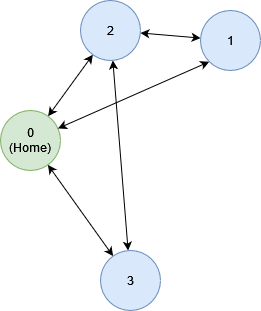
\includegraphics[width=.5\textwidth]{automatos.png}
\caption{Movimentação do Drone Entre as Bases}
\label{fig:Movimentos do Drone}
\end{figure}

Em relação ao carregamento, o drone possui capacidade para carregar \textbf{ou} um container \textbf{ou} até 3 amostras. Ele pode carregar e descar regar livremente, contanto que respeitando seus limites de carga. Assim, a sequência. Cada amostra é coletada e guardada individualmente, permitindo que, por exemplo, sejam coletadas na área de uma base e armazenada em outra. Por fim, para que ele possa desligar-se, não pode estar carregando nada (todo item carregado deve também ser descarregado ao longo da execução). 

\section{A Linguagem}

Para definir uma linguagem capaz de modelar o sistema, primeiro definiremos o alfabeto, que consistirá dos comandos que o drone poderá receber.


\begin{itemize}
  \item \textit{\textless Base0\textgreater}, \textit{\textless Base1\textgreater}, \textit{\textless Base2\textgreater}, \textit{\textless Base3\textgreater} - Move o drone para a base indicada.
  \item \textit{\textless LoadBox\textgreater} - Carrega o drone com o container, ocupando toda sua capacidade de carga.
  \item \textit{\textless UnloadBox\textgreater} - Descarrega o container, liberando sua carga.
  \item \textit{\textless CollectSample\textgreater} - Coleta uma amostra, ocupando um dos seus três espaços de carga.
  \item \textit{\textless StoreSample\textgreater} - Guarda uma das amostras que está carregando, liberando um de seus três espaços de carga.
  \item \textit{\textless Shutdown\textgreater} - Desliga o drone, encerrando a sequência de instruções. Só pode ser executado se o drone estiver na base 0 e sem carregar nada, como a última operação.
\end{itemize}

A fim de facilitar a interação com o sistema, também é conveniente que o sistema informe como saída, após cada operação, a base e carga atuais do drone, em caso de sucesso ou um erro explicativo, em caso de falha na execução.

Exemplos de saída em caso de sucesso:
\begin{itemize}
    \item \texttt{Base: 0 $\mid$ Carga = [...]};
    \item \texttt{Base: 1 $\mid$ Carga = [II.]};
    \item \texttt{Base: 3 $\mid$ Carga = [XXX]};
\end{itemize}

Exemplos de saída em caso de erro:
\begin{itemize}
    \item \texttt{\textbf{Erro: Movimento inválido}};
    \item \texttt{\textbf{Erro: Carga excede o limite}};
    \item \texttt{\textbf{Erro: Desligamento fora da "Home"}};
\end{itemize}

Um detalhe interessante sobre a linguagem é o fato de que, apesar de, inicialmente, a linguagem aparentar requerer diversos duplo-balanceamentos (a fim de gerenciar o sistema de carga e descarga), como a quantidade de possibilidades para os valores de carga é finita, é possível reconhecê-la usando um Automato Finito Determinístico, como o mostrado abaixo.

\newpage

\begin{figure}[ht]
\centering
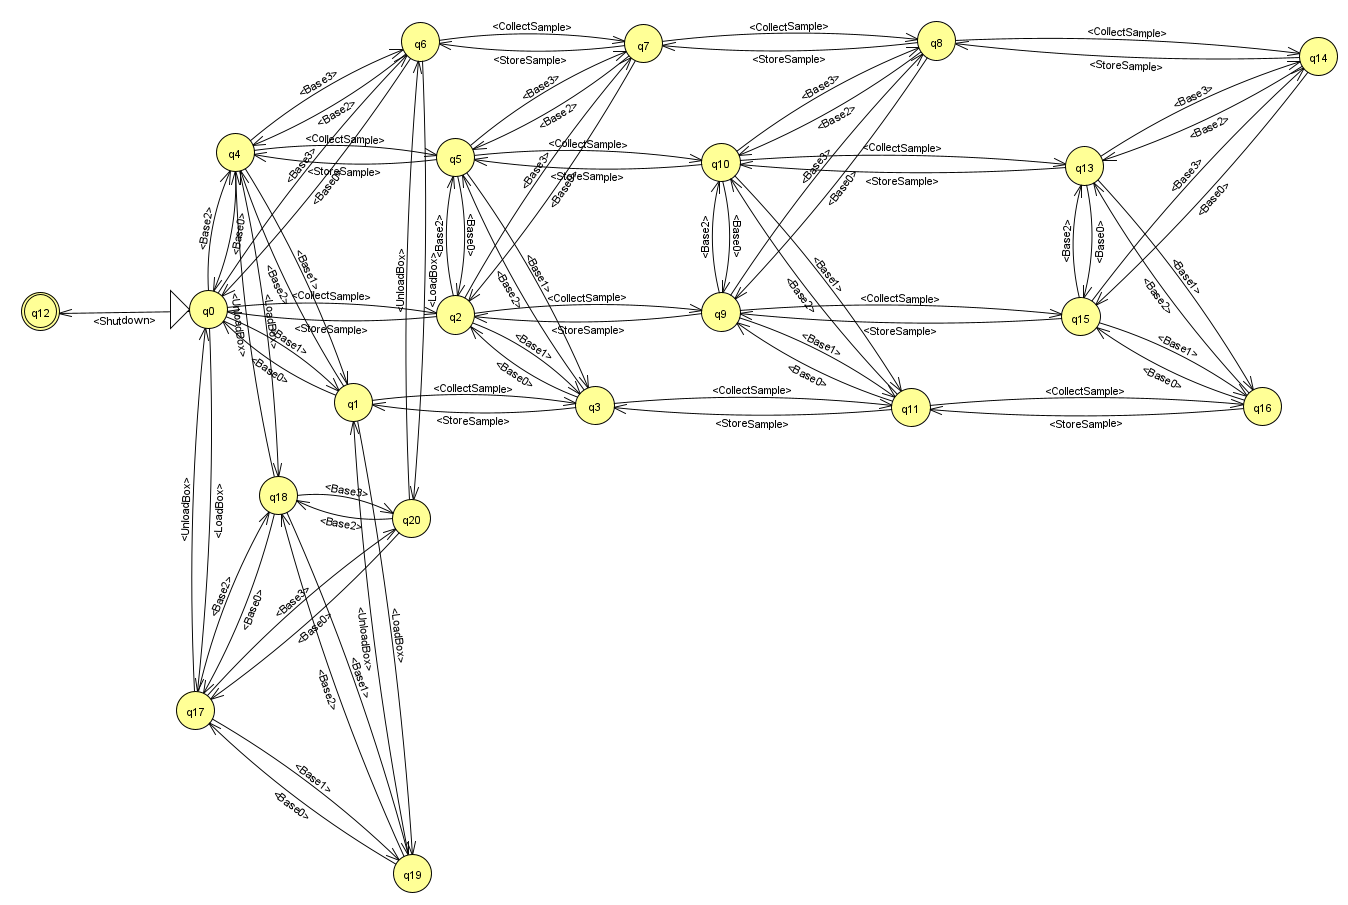
\includegraphics[width=\textwidth]{automato.png}
\caption{Automato Reconhecedor da Linguagem}
\label{fig:Automato Reconhecedor}
\end{figure}



Apesar de parecer complexo, o autômato acima basicamente opera através de um simples autômato capaz de reconhecer os movimentos do drone pelas bases, copiado para cada uma das possíveis cargas: vazio, 1, 2 ou 3 amostras, ou um container.

\end{document}
